Numerical wave models are used for a wide variety of applications. These include 
navigation safety, ocean engineering for marine energy (oil and gas or renewables) or ship design, coastal engineering. 
Wave models are used both for forecasts and hindcasts, for deterministic simulations or ensemble predictions. 

Because waves also have impacts on 
the atmosphere, ocean, sea ice, or sediments, wave models are increasingly used in Earth System models, coupled with other dynamical models. 
This coupling is most important in shallow waters (storm surges, wave-driven currents ...) and specific 
aspects of coastal and shallow water wave modelling will be discussed in chapter \ref{ch_model_coastal}. Our purpose here is to give indications about the 
validity and limitations of wave models. As we focus on deep water, it removes the specific issues of bottom friction, refraction, shoaling, 
making the question of wave evolution more simple. The first question to consider is: what is deep water?  From chapter \ref{ch1b}, the 
ratio of the wavelength and water depth represented by $kD$, is one criteria. Typically when $kD > 2$ the effect of shoaling and refraction can 
usually be neglected. 

This chapter only deals with spectral phase-averaged models, based on the wave action equation (\ref{Action_balance}), 
following the first numerical model of \cite{Gelci&al.1957}.  The practical problem is to obtain the most accurate result, either for 
a forecast for the coming days a climate projection over long terms, or a restrospective simulation (hindcast), using limited 
computational resources and time. This leads to trade-offs between expensive calculations, for example the 4-wave interactions, 
and cheaper parametrizations. The choice of the numerical method also has a strong impact on the model cost, with benefits that may be visible 
only for some parameters. 

What are the main factors that control the model accuracy?
\begin{itemize}
\item Because waves are generated by winds, and propagate in a medium characterized by a bottom topography, currents and obstacles (small islands, sea ice ...), 
the quality of these forcing fields is determinant, and the accuracy of winds is certainly the most important. 

\item  The second most important factor is the accuracy and behavior of the parametrizations use for all the processes represented 
in the source terms $S$ in eq. (\ref{Action_balance}). These parameterizations should be \emph{robust}, meaning that they should work under all circumstances from 
calm seas to hurricane-force winds, in the presence or absence of swells ...  Many model errors can be traced to poor parametrizations.  No parametrizations is perfect
but some definitely produce more accurate results than others. 

\item Finally, there is no method to solve eq. (\ref{Action_balance}) to the accuracy of the computer round-off error at an acceptable computational cost. 
The numerical integration methods 
are thus based on approximations that lead to numerical diffusion. Also, numerical limiters in the evolution are used by many models, 
so that the numerical result may be very different from the actual solution of the wave action equation \citep[e.g.][]{Tolman2002b}. 
One infamous example is the effect of semi-implicit integration of the source terms in time when large time steps are used 
\citep{Hargreaves&Annan2000}. This particular issue motivated the use of an adaptative time step for source term integration in the 
WAVEWATCH III model \citep{Tolman&al.2014}. 
\end{itemize}

The overall model quality is thus the result of many choices. As a user, you should be very careful about supposedly `default' model settings:
this means that somebody has chosen for you, however reasonable 
that choice may be in usual conditions, it may be not be the best choice for your particular application.  
As a user of a wave model you may not have the freedom to choose, and the choice of model or forcing may be imposed because it is more or less easily available 
and easy to use. Whatever the circumstances, you should be aware  of the impact on the model results. 
Also  you may end up frustrated by model result that exhibit unphysical behavior: such as the stronger growth of wind sea in the presence of swell or 
a broadening of  the directional wave spectrum in shallow water. You  may thus want 
to try yourself and improve on the existing models. Hopefully the next sections will be interesting advice. As for the swell effect of wind growth, 
we have not get a full physical model that would give the proper reduction in wind sea growth \citep{Garcia&al.2012}, but at least, 
going from the parameterization by \cite{Janssen&al.1994} to the one by \cite{Ardhuin&al.2010} you will not see anymore the 
wind sea wave height jump up when swell arrives. 

As mentioned, the most important choices that define the model accuracy are the model forcing, model parametrizations, and numerical schemes. 
 Models may also assimilate measurements to correct past estimates of the waves. However, contrary to atmospheric or oceanic circulation models, 
 assimilation is not necessary to obtain accurate forecasts and hindcasts. 
For all these choices, the most accurate result is not necessarily obtained with the most complex choice, because some errors are often 
compensated by other errors. 

Finally, models are usually good only for the parameters for which they have been validated, and for the ranges of these parameters in which we have data. 
Remember that there are very few measurements of the full frequency-direction 
spectrum, so that the modeled spectral shapes can be really bad, especially at high frequencies. When one predicts that the 100-year significant wave height 
off the west coast of France is 18~m, based on a model that has only been validated up to 14~m, this is a real extrapolation. 


\section{Forcing}
\subsection{Bathymetry and islands}
If you have never run a numerical wave model, it probably sounds trivial that the ocean depths and shape of the shoreline should be known. In practice, 
though, it is not always easy. Global databases such as ETOPO \citep{Sloss1993} and GSHHS \citep{Wessel&Smith1996} can have important errors, with large 
error in water depth over continental shelves, and some islands
misplaced by a few kilometers. Even at global scales and coarse resolutions, it is important to take into account subgrid islands such as the Tuamotus or Aleoutian 
islands in the Pacific \citep{Tolman2003}, as illustrated in figure \ref{fig_obstruction}.

%%%%%%%%%%%%%%%%%%%%%%%%%%%%%%%%%%%%%%%%%%%%%%%%%%%%%%%%%%%%%%%%%%%%%%%% figure
\begin{figure}
\centerline{\includegraphics[width=0.7\textwidth]{FIGS_CH_MODEL/Chawla_obstruction.pdf}}
%\vspace{3.64in}
\caption{Left picture: example of wave attenuation due to propagation across many islands, here the Tuamotus, for a case of swell from the 
North-East, which almost never happens in this region, as computed on a 3.6~km grid. These islands  
would not be resolved in a typical ocean global grid \citep[reproduced from][]{Chawla&Tolman2008} and require a sub-grid parameterization as 
introduced by \cite{Tolman2003}. The dashed box corresponds to the extent of the right panel 
which shows the mean values of $H_s$ recorded by TOPEX and Jason (reproduced from \cite{Andrefouet&al.2012}, showing the very strong sheltering in 
real conditions with both windsea and swell, with swell usually coming from the South-West.}
\label{fig_obstruction}
\end{figure}
%%%%%%%%%%%%%%%%%%%%%%%%%%%%%%%%%%%%%%%%%%%%%%%%%%%%%%%%%%%%%%%%%%%%%%%% figure

\subsection{Wind fields: analyses, forecasts, re-analyses}
Although there are many measurements of surface winds based on satellite radiometers or scatterometers, the coverage they provide is not 
enough to use a forcing field defined from these data only. Hence it is most common to use winds from an atmospheric circulation model. In these models, 
the near-surface wind speed, usually 10 meters, is not a an dynamical parameter because these models usually have a vertical discretization in pressure 
levels that does not follow a constant height. This surface wind, possibly corrected for stability effects 
in the form of a \emph{neutral}
wind, is in fact diagnosed from the atmospheric boundary layer parameterization. 
As a result there are significant differences between models. For example, for wind speeds 
exceeding 30~m/s, the winds provided by the European Center (ECMWF) as part of their operational analyses were typically 10\% slower than those of the U.S. weather 
service (NCEP) for the year 2005.
Given that there are very few reliable data at high wind speeds, it is difficult to decide which is more accurate
correct. As a result, the wave model parameterizations are adjusted differently to the different forcing fields. 

If you are a scientist, you will probably try to get the most accurate wind fields. If you are an engineer, you may be in a rush or may not have 
access to the most accurate database. When it comes to wind vectors, the most accurate model analyses and forecasts over the recent years and 
most of the globe, are those provided by the European Center for Medium Range Weather Forecasting (ECMWF). 
Although their data policy may soon change, these are usually not freely available. The anlysis is the combination of model and observation that 
is expected to produce the most accurate estimate of the state of the atmosphere, providing the initial conditions from which the forecast in produced. 

ECMWF, like most Numerical Weather Prediction 
(NWP) organizations, produces both deterministic analyses and forecasts, a single simulation, and ensemble predictions, which consist of a set of 
simulations that is designed to explore the possible variations of the atmospheric state. ECMWF spatial resolution of the deterministic product 
was reduced to 0.25 degree in 2008,  0.125 
degree in 2011, and 9~km in March 2016. Their system, like those at all NWP centers is constantly improving to take the best advantage of computer power, 
new observations, new model parametrizations and assimilation methods. 

You may find details about ECMWF's Integrated Forecasting System (IFS) on their website with a nice quarterly newsletter. 
It can be a good idea to check on the quality of other sources by looking at the wind and wave model verification 
%\url{http://www.jcomm-services.org/Wave-Forecast-Verification-Project.html}, 
\href{http://www.jcomm-services.org/Wave-Forecast-Verification-Project.html}{\small{http://www.jcomm-services.org/Wave-Forecast-Verification-Project.html}}, 
presented by \cite{Bidlot2008}.

Wind analyses and deterministic forecasts have made enormous progress over the last 20 years \citep[e.g.][]{Janssen2008a}, 
thanks to an increase in computational power that allows higher resolution, more complex parameterizations and 
sophisticated data assimilation. This has gone with a dramatic increase in number and quality of observations. 
Figure \ref{fig_wind_quality} shows the reduction in errors in both analyses and forecasts for winds speeds and wave heights in ECMWF 
operational deterministic forecasting system. 
%%%%%%%%%%%%%%%%%%%%%%%%%%%%%%%%%%%%%%%%%%%%%%%%%%%%%%%%%%%%%%%%%%%%%%%% figure
\begin{figure}
\centerline{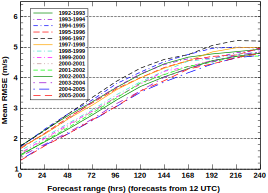
\includegraphics[width=\textwidth]{FIGS_CH_MODEL/wind_quality_v2.pdf}}
%\vspace{3.64in}
\caption{Root mean square error (RMSE) as a function of the forecast range, 0 corresponding to the analysis, in the operational systems ran 
at ECMWF. These modeled wind speed and wave heights are compared to buoy measurements over a year centered in winder 
(August to July). Only every other year is shown (Picture courtesy of J. Bidlot).}
\label{fig_wind_quality}
\end{figure}
%%%%%%%%%%%%%%%%%%%%%%%%%%%%%%%%%%%%%%%%%%%%%%%%%%%%%%%%%%%%%%%%%%%%%%%% figure

Because of this continuous improvement of model quality, a time series of operational hindcasts is not homogeneous in time. Hence, 
a statistical analysis of extreme events based on operational analysis will probably have spurious trends. In order to reproduce 
past events as well as possible, recent versions of the atmospheric models have been re-run to produce re-analyses. In this case 
the only source of non-homogeneities are the observations assimilated. It is indeed not possible to go back in time and add a few satellites. 
For this reasons, some atmospheric reanalyzes start in 1978, when enough satellite data is available for a reasonable estimate of the 
atmospheric circulation. This is the case of the Climate Forecast System Reanalysis  \citep[CFSR][]{Saha&al.2010} 
and ERA-Interim \citep{Dee&al.2011}. Other re-analyses go back to 1958 \citep{Kobayashi&al.2015}, and \cite{Compo&al.2011}
 have produced a re-analysis from 1871 to 2008.
 
As we have seen, the highest waves require very high winds, and the quality of re-analyses for estimating past wave heights critically depends 
on the capability of the atmospheric models to resolve the gradients in small storms, in particular for tropical storms or polar lows. As a result, some wave re-analyses like ERA40 are notorious for understimating 
wave heights because of underestimated winds \citep{Caires&Sterl2005}. Unfortunately for that aspect, the more recent fitfh generation re-analysis (ERA5) at ECMWF 
favored an ensemble approach, rather than single and higher resolution model \citep{Hersbach&al.2020}. The ERA-5 winds are likely biased low for wind speeds above 21 m/s \citep{Pineau-Guillou&al.2018}. A monthly report on wind and wave model accuracy can be found here \url{https://confluence.ecmwf.int/display/WLW} .
 

\subsection{Coastal winds}
In coastal regions, closed or semi-closed basins surrounded by mountains, such as the northern Mediterranean, the winds 
from global models are often inaccurate due to a lack of resolution of the land topography that channels winds. 
A striking view of this is in figure 
\ref{wind_Cavaleri} \citep{Cavaleri&Bertotti2006}. In this case, a solution can be to use higher resolution local area models. 
However, it must be noted that the quality of the nested grid result, owes much to the boundary conditions and 
the quality of the parent model. Sometimes a statistical correction of coarse grid can be a better option \citep{Signell&al.2005}.
%%%%%%%%%%%%%%%%%%%%%%%%%%%%%%%%%%%%%%%%%%%%%%%%%%%%%%%%%%%%%%%%%%%%%%%% figure
\begin{figure}
\centerline{\includegraphics[width=\textwidth]{FIGS_CH_MODEL/Cavaleri_Bertotti_U10_Hs.pdf}}
%\vspace{3.64in}
\caption{Average wind and wave height in the Northern Hemisphere, Southern Hemisphere and Mediterranean sea, 
obtained in different runs of the ECMWF model in which the spatial resolution is changed. The resolutions of Gaussian grids 
T106, T213, T319, T511, T639, et T799 correspond to 
188, 94, 63, 39, 31, and 25~km. Wind speed and wave height values have been divided by the values obtained for the coarsest 
of these grids. Taken from \cite[][\copyright Elsevier]{Cavaleri&Bertotti2006}.}
\label{wind_Cavaleri}
\end{figure}
%%%%%%%%%%%%%%%%%%%%%%%%%%%%%%%%%%%%%%%%%%%%%%%%%%%%%%%%%%%%%%%%%%%%%%%% figure

\subsection{Observed winds}
Winds over the oceans are measured by altimeters, scatterometers (or their higher resolution cousins, SARs) and radiometers with increasing 
coverage and accuracy. It is now possible to have data everywhere over the oceans at a resolution of about 12~km, and every 12 hours. 
Although 12 hours is long compared to the time scale of evolution of the wind fields and we cannot use this data as such to force a wave model, 
it is possible to blend this with atmospheric models to improve the realism of modelled winds \citep[e.g.][]{Bentamy&al.2007}. 

Although some of that data is assmilated into atmospheric models, these models often reject the highest winds that are often too far from their 
first guess. As a result, it is always a good thing to check the consistency of modeled winds against data. Although traditional scatterometers that use Ku or C 
are not able to discriminate wind speeds beyond 25 m/s, the use the measured Doppler shift \citep{Mouche&al.2012} or cross-polarizations \citep{Vachon&Wolfe2011,Mouche&Chapron2015}, 
has been demonstrated with SAR data to be able to better constrain higher wind speeds, and will be used in future scatterometers. The recent use of L-band, which is more 
sensitive to longer waves than Ku or C, has also been shown to be sensitive to the highest wind speeds \citep{Reul&al.2012}. 

\subsection{Currents}
The main issue with ocean currents is to get accurate estimations of current fields, at the relevant resolution \citep{Ardhuin&al.2017a}. This is relatively simple for tide-dominated environment 
for which numerical models are reasonably goog \citep[e.g.][]{Ardhuin&al.2012}, it is much more delicate for regions dominated by quasi-geostrophic dynamics, where 
deterministic ocean circulation forecasts have limited skills, 
and even more so where internal waves are the main source of surface current gradients \citep{Osborne&Burch1980} due to the required high resolution to resolve these 
features.  As a result, most operational wave forecasting systems take into account tidal currents, at best. 

\subsection{Sea ice}
Wave-ice interaction is the topic of chapter \ref{ch_ice}. To summarize it here, the presence of ice has a strong impact on wave growth and disspation, and a knowledge of ice concentration  
is required in any ocean basin that has some ice, the Arctic of course, but all three oceans (Atlantic, Indian and Pacific) are strongly influenced by ice, at least 
in their southern hemisphere part, and many regional seas an lakes also freeze up: the Baltic, Caspian, the Great Lakes...  Experimental evidence shows 
that waves are not generated by the wind in ice-covered regions, and the ice can damp the waves very rapidly, in particular the high frequency components.

\section{Numerics}
\subsection{Wave models are big}
The problem of numerical wave modelling at oceanic scales is often a question of compromise between spectral and spatial resolution. Indeed, our wave action spectrum 
is a 4-dimensional beast that we have to integrate in time. All models today use a fixed discretization into $N_f \simeq 30$ frequencies and $N_\theta \simeq 30$ directions. 
The wave action equation \ref{Action_balance} is thus a set of $N_f \times N_\theta \simeq 1000$ hyperbolic advection equations that are coupled via the source term $S$ and the 
refraction and shoaling terms. Each equation for a component $(f_i,\theta_j)$ is a 2-dimensional partial differential equation (PDE) that represents advection equation with source term.  This is a fairly standard problem to 
solve, with the transport velocity $\Cb_g + \Ub$ varying in space and possibly in time. If the spatial discretization is a regular mesh with only  100 by 100 points, 
hence a spatial discretization into 10,000 nodes, the overal problem has 10 million unknowns: all the values of our gigantic wave action matrix. As result, wave models typically 
use a lot of memory. For example at ECMWF, with the IFS system, the wave model uses about as much as the entire atmosphere. 

Now, every time I think of it, it makes me mad that most of these unknowns are zeros: waves over 25~s period do not happen very often, but they do happen once in a while in the 
biggest storms \citep{Hanafin&al.2012}. One trick could be to adjust the spectral grid to remove the components for which we have zeros on the entire grid or in a subgrid. 
At the same time, the recent extension of wave models to add shoreline reflections \citep{Ardhuin&Roland2012} and sources of low-frenquecy infragravity waves  \citep{Ardhuin&al.2014} have 
replaced these zeros by small numbers that can be significant for some applications.
Still, if you do not activate these options, there should be a way to make models faster by avoiding to compute zero plus zero times zero equals zero.

\subsection{Spectral discretization}
In frequencies, one needs to choose 
\begin{itemize}
 \item the spacing between frequencies: it is usualy exponential, with $f_{i+1} = X_{fr} f_i$ where  $X_{fr}$ is a constant close to 1.1. The reason for this geometric 
 progression is that it simplifies the calculation of the 4-wave interaction term $S_{nl}$: in deep water the geometric 
 arrangement of the interacting waves is the 
 same from one frequency to the next. The choice of $X_{fr}=1.1$ is relatively coarse, as a JONSWAP spectrum will 
 have only one or two frequencies inside of the peak. However, 
 going to $X_{fr}=1.05$ will double the number of frequencies, if you used 30 it now jumps to 60, and double the 
 cost of the model.  
 \item a minimum frequency $f_{\min}$: this should be low enough to allow waves to develop. In the open ocean, 
 it is possible to get a peak period of 25~s \citep{Hanafin&al.2012},
 and you probably need a couple of frequency bands below that to allow the spectrum to roll back, this  means 
 that $f_{\min}=0.037$~Hz may already be too high.  
 \cite{Ardhuin&al.2014} have also gone as low as 0.003~Hz to model the infragravity part of the spectrum 
 which will be discussed in chapter \ref{ch_surf}. However, adding these 
 frequencies means using a lager number $N_f$ of frequencies, and also the computation cost for these low 
 frequencies can be higher due to numerical constraints: these 
 long period waves have larger group velocities, and explicit 
 schemes will require a smaller time step. 
 \item a maximum frequency $f_{\max}$, this is dictated by the lowest winds that you want to represent 
 properly: to catch the peak of the wind sea 
 you need to have  $f_{\max} > 1.2 {X}_{fr} g/(2\pi U_{10})$. For a fairly frequent wind speed of 5 m/s, 
 this means that $f_{\max} \simeq 0.4$~Hz is not enough. Still, 
 this was used  recently in many global models. Also, if you want to investigate properties of high 
 frequency waves or backscatter for remote sensing, you probably want 
  $f_{\max} > 0.7$~Hz. Finally, most wave model ignore viscous dissipation \citep{Dore1978} and capillary effects. These cannot be ignored for  $f_{\max} > 2$~Hz.
\end{itemize}
%%%%%%%%%%%%%%%%%%%%%%%%%%%%%%%%%%%%%%%%%%%%%%%%%%%%%%%%%%%%%%%%%%%%%%%% figure
\begin{figure}[htb]
\centerline{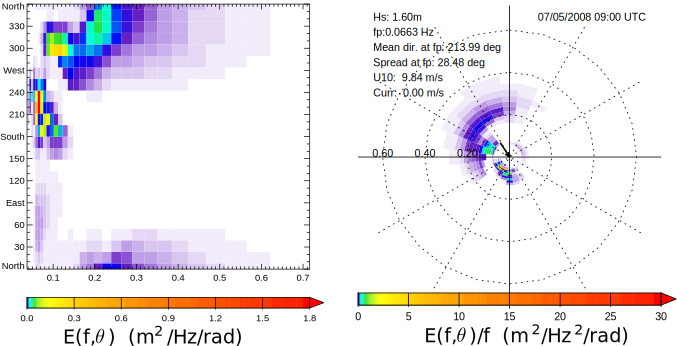
\includegraphics[width=0.8\textwidth]{FIGS_CH_MODEL/spectrum_discrete.pdf}}
%\vspace{3.64in}
\caption{Example of spectral discretization: here these modeled spectra use 32 frequencies from 0.037~Hz to 0.72~Hz with $X_{fr}=1.1$, and 24 directions. The same spectrum 
is shown in cartesian and polar coordinates. 
Note that the polar representation is nice to show the waves in the direction from where they are arriving, but it squeezes all the dominant waves near the center, 
making it difficult to see the details. Here the spectrum in polar coordinates is divided by the frequency $f$ which compensates a little for the squeezing: the 
total energy is still the area in the plot times the value plotted.}
\label{fig:sectral_discretization}
\end{figure}
%%%%%%%%%%%%%%%%%%%%%%%%%%%%%%%%%%%%%%%%%%%%%%%%%%%%%%%%%%%%%%%%%%%%%%%% figure
For the directions, with a directional spread that is about 20$^\circ$ for the wind sea peak, a 
resolution of 15$^\circ$ (i.e. 24 directions), can be satisfactory with 2 points in the peak  -- the spread is the half-width of the spectrum in the 
limit of a narrow Gaussian shape. 
As wind-waves turn into swell, the spread can be as low as  5$^\circ$, 
and it can be useful to have a higher directional resolution. Again this comes at a cost: 
more direction means larger spectra, more memory and computational time. 



\subsection{Spatial discretization}
Given the cost induced by spectral discretization, the spatial discretization can be optimized in several ways. 
First of all, one should consider the necessary resolution. In the absence of currents, the gradients in the wave field are given by the 
wind field and the shoreline geometry. There are thus several options, from a regular grid in latitude and longitude to a triangle-based mesh
\citep[e.g.]{Benoit&al.1996,Roland&Ardhuin2014}, or mosaics of grids with different resolutions \citep{Tolman2008} or quad-trees \citep{Popinet&al.2010,Li2010}. 
In particular, high resolution is desirable in hurricanes, and moving or adaptive grids have thus been designed for this \citep{Tolman&Alves2005,Popinet&al.2010}. 
All these options are available in the WAVEWATCH III modelling framework. 

\subsection{Integration methods}
There are two large classes of methods used for this type of multi-dimensional PDE. 

\begin{itemize}
\item a global resolution with an iterative method: a method of lines as described in e.g. \cite{Patankar1980}. Here, all terms of the equation are discretized first and thereafter integrated in time using an ODE solver. This method has been applied in the SWAN model \cite{Booij&al.1999}. Since the equation is rather stiff a fully implicit scheme is commonly employed for the time integration. In turn, due to nonlinear source terms, this is accompanied by an iteration process. 
\item  A splitting method following \cite{Yanenko1971}. In that case the several terms of the equation are integrated in succession, 
\begin{eqnarray}
 \frac{\partial N}{\partial t} &+& \mathrm{advection} = 0 \\
 \frac{\partial N}{\partial t} &+& \mathrm{refraction} = 0 \\
 \frac{\partial N}{\partial t}  &=& S/\sigma.
\end{eqnarray}
In the limit of small time steps, this is equivalent to the full integration. This approach is used in 
WAM \citep{WAMDI1988}, and for most options of WAVEWATCH III \citep{Tolman2002d}, and in TOMAWAC the first two steps are combined 
\citep{Benoit&al.1996}.
\end{itemize}

The first approach can be interesting at very high resolution, typically in the nearshore, when used with implicit methods that 
are not constrained to have very small time steps. It is used in SWAN \citep{Booij&al.1999} and has been implemented in a research version of WAVEWATCH III \citep{Huchet&al.2015}.  

The great benefit of the second approach, is that the splitting allows to adapt the time step to the time scale of evolution of 
each term. This is fully used in WAVEWATCH III, with an adaptative time step for the source term integration, and different time steps
for the advection and refraction. 

In order to limit the computational time to something acceptable, wave models use limiters: the rate of change of evolution 
is limited to ensure stability while keeping large time steps. These limiters can completely change the solution \citep{Tolman2002b,Roland&Ardhuin2014}, so that it 
is a good practice to test that a model gives similar results when reducing all time steps by a factor 2. When 
a splitting approach is used, different limiters  can be applied to different pieces of the equation. For example, WAVEWATCH III has a limiter on refraction (waves cannot 
turn by more than $\Delta_\theta=2\pi/N_\theta$ over one refraction time step $\Delta_{t,r}$: if the bottom slope of current gradient require a faster rotation then the 
rotation speed is limited to  $\Delta_\theta/\Delta_{t,r}$. Limiters for source term integration are a bit more complex.  

\subsection{Source term integration}
The source terms link all spectral components together, including high frequencies that can evolve very fast. For that reason and also because the source term balance
$S_{\mathrm{in}}+S_{\mathrm{nl}}+S_{\mathrm{ds}}$ is generally not well reproduced at high frequencies by parameterizations \citep[e.g.][]{Zieger&al.2015}, 
the spectrum above a diagnostic frequency $f_d$ is usually prescribed to decrease like $f^{-5}$. This cannot reproduce the observed broadening of the directional
spectrum with increased frequencies \citep[e.g.][]{Banner&al.1989,Leckler&al.2015} but it is a shortcut to keep the models within reasonable bounds. 
In the ECWAM model 
$f_d$ is set to be the maximum of 2.5 times the mean frequency of the wind sea and 3 times the Pierson-Moskowitz frequency \citep{Bidlot2012}.

A stable integration of the source terms is possible with an implicit integration, 
\begin{equation}
 N(t+\Delta_t) = N(t) + \frac{S(t) \Delta_t}{\sigma(1 -   \alpha \Delta_t \partial S/\partial N / \sigma)}.
\end{equation}
With $ \alpha = 0.5$ this is accurate to second order in time, but $ \alpha = 1$ generally performs better for the short 
wave components \citep{Hargreaves&Annan2000}. Still, one should be careful that source term integration is sensitive to the choice of time step it if is constant. 
As a result, even at frequencies $f < f_d$, a limiter is used for spectral evolution. The design of this limiter is discussed in \cite{Tolman2002b}. 


\subsection{Spatial propagation}
The early wave models such as WAM \citep{WAMDI1988} have chosen the cheap but robust first order 'upwind' scheme. 
In only one dimension, the wave propagation direction is given by a sign $s$, going towards $x>0$ if $s=1$ and in the opposite direciton if $s=-1$. The 
upwind advection scheme is thus 
\begin{eqnarray}
 N(x,t+\Delta_t) & =&  N(x,t) - \frac{\Delta_t}{\Delta_x} \left[ C_g(x) N(x) - C_g(x-\Delta_x) N(x-\Delta_x,t) \right] \quad \mathrm{if} \quad s =1 \\
N(x,t+\Delta_t) & =&  N(x,t) + \frac{\Delta_t}{\Delta_x} \left[ C_g(x+\delta_x) N(x+\delta_x) - C_g(x) N(x,t) \right] \quad \mathrm{if} \quad s=-1. 
\end{eqnarray}
The name upwind expresses the idea that the information is taken from  where it is coming. That scheme is stable when the Courant number 
$C_g \Delta_t/\Delta_x$ is less than 1. This condition is known as the CFL condition after the work of Courant, Friedrichs and Lewy \citep{Courant&al.1928}.
%%%%%%%%%%%%%%%%%%%%%%%%%%%%%%%%%%%%%%%%%%%%%%%%%%%%%%%%%%%%%%%%%%%%%%%% figure
\begin{figure}[htb]
\centerline{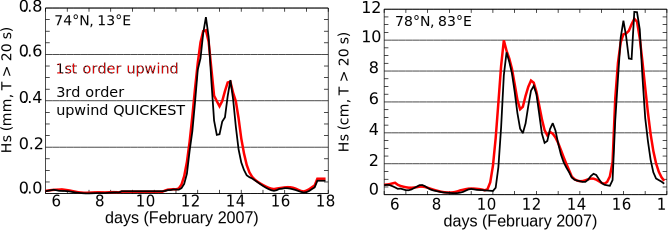
\includegraphics[width=0.8\textwidth]{FIGS_CH_MODEL/PR1_UQ_timeseries.pdf}}
%\vspace{3.64in}
\caption{Time series of modeled wave height (computed over wave periods longer than 20~s) at two locations of the Arctic, using 
the first order upwind scheme, or 
the third order upwind QUICKEST scheme - including the Garden Sprinkler Effect correction of  \cite{Tolman2002a}.}
\label{fig:PR1_UQ_time}
\end{figure}
%%%%%%%%%%%%%%%%%%%%%%%%%%%%%%%%%%%%%%%%%%%%%%%%%%%%%%%%%%%%%%%%%%%%%%%% figure

The main defect of the first order upwind scheme is its large numerical diffusion: a localized packet of energy tends to disperse in space. This 
dispersion effect is not always bad because real waves are dispersive, but the physical dispersion is only a function of the spectral resolution. 
A much reduced diffusion can be obtained by using higher order schemes, such as the third order upwind QUICKEST scheme of \cite{Leonard1991}.
This is obvious in figure \ref{fig:PR1_UQ_time}, which shows time series of wave heights
in the ice-free part of the Arctic, in February 2007. The two biggest storm of the year in the North Atlantic occured on February 9 and 10, 
sending swell to the Arctic. This swell is modeled to arrive on 13 and 14 February off the East coast of Greenland at (74$^\circ$N,13$^\circ$W), 
and the two peaks are less separated with the first order than with the third order scheme. Things are worse as waves propagate further, and the 
two peaks are almost indistinguishable north of Siberia on February 16 and 17, at (78$^\circ$N,83$^\circ$E). As a result, the investigation of the potential diffusion 
effect of sea ice on these swells \citep{Ardhuin&al.2016} would not be possible with a first order scheme. That first order scheme is still used 
at ECMWF. 

%%%%%%%%%%%%%%%%%%%%%%%%%%%%%%%%%%%%%%%%%%%%%%%%%%%%%%%%%%%%%%%%%%%%%%%% figure
\begin{figure}[htb]
\centerline{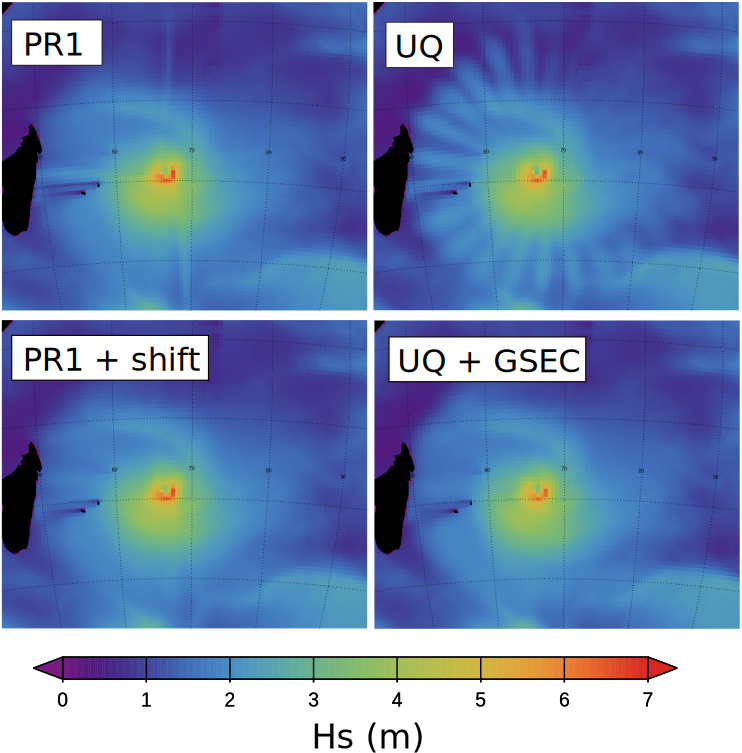
\includegraphics[width=0.7\textwidth]{FIGS_CH_MODEL/PR1_UQ_cyclone.pdf}}
%\vspace{3.64in}
\caption{Example of wave heights for Tropical Cyclone Dora, in the Southern Indian ocean, using 4 different numerical schemes. 
'GSEC' is the GSE correction scheme of 
\cite{Tolman2002a}. All model runs use 24 directions. }
\label{fig:PR1_UQ_space}
\end{figure}
%%%%%%%%%%%%%%%%%%%%%%%%%%%%%%%%%%%%%%%%%%%%%%%%%%%%%%%%%%%%%%%%%%%%%%%% figure
It is also troubling that the mean values are different, because the diffusion in the first order scheme strongly depends on the orientation relative to the 
grid: the discrete directions that travel along the grid axis are much less diffused. This shows up as north-south beams of energy in the case
of slowly moving storms, such as Tropical Cyclone Dora, shown in figure \ref{fig:PR1_UQ_space}. To reduce that effect, the usual trick is to shift 
the directions by $\Delta_\theta/2$: instead of using 0, 15$^\circ$, 30$^\circ$ ... one uses 7.5$^\circ$, 22.5$^\circ$, 37.5$^\circ$ ... 
Now, instead of a maximum along the meridian, we get a weak minimum (see top-left and bottom-left 
panels in figure \ref{fig:PR1_UQ_space}). 


When numerical diffusion is strongly reduced, the dispersion of the wave field can be less than expected from the physical dispersion, giving 
an anomalous effect of the spectral discretization, known as 
the `garden sprinkler effect' (GSE). Without any GSE correction, the upwind QUICKEST scheme gives the beautiful flower pattern in 
figure \ref{fig:PR1_UQ_space}: because each spectral component has its own speed and direction, waves from a very small source separate as they 
propagate away from the source as discrete blobs of energy, instead of a smooth pattern that would be obtained with a very fine spectral 
discretization in frequency and direction. The solution to correct this GSE is to introduce some explicit diffusion \citep{Tolman2002a}.

Such differences are much less visible for fast moving storms, such as the more powerful cyclone Gamede which struck La Reunion island 
on February 25. 


\section{Parameterizations of physical processes}
Because of the complexity of wave evolution processes that were briefly described in chapter \ref{ch_sourceterms}, and further discussed Part 3, there is no generally agreed upon parameterization for wave generation and dissipation. Also, the non-linear 
wave interaction that is based on the theory of \cite{Hasselmann1962} is too costly to be computed accurately for routine applications. Hence several 
parameterizations have been proposed to reproduce the non-linear source function. The most common is the Discrete Interaction 
Approximation by \cite{Hasselmann&al.1985b}, which keeps the energy, action and momentum conservation properties of the full non-linear interaction, 
at the price of an overestimation of the flux of energy to high frequency, among other side effects. 

For wave generation and dissipation, the parameterizations proposed by the \cite{WAMDI1988}, \cite{WAMBook}, \cite{Tolman&Chalikov1996}, 
\cite{Banner&Morison2006},  \cite{Ardhuin&al.2010}, 
\cite{Rogers&al.2012}, and many others, have tried to represent the magnitude of the wind to wave energy and momentum fluxes, as well 
as the overall balance that gives the wave growth. We cannot describe here in details all the flavours of the proposed parameterizations, nor 
give all details about their impact in the model solutions, which is the topic of an abundant record of scientific publications. We will try to 
summarize what we believe to be the most salient aspects and side effects of a few common parametrizaion, looking here only at the resulting 
wave spectra and derived parameters. In the context of coupled models (wave-atmosphere or wave-ocean or wave-sea ice...) one should probably focus more 
on the fluxes of energy and momentum than on the shape of the wave spectrum. This will be discussed in chapter \ref{ch_ioa}. 


What follows is mostly taken from a few recent papers by \cite{Rascle&Ardhuin2013}, \cite{Roland&Ardhuin2014} and \cite{Stopa&al.2016c}, and
focuses on large 
scale oceans away from the ice-covered regions. Modelling in and around ice-covered regions will be discussed in chapter \ref{ch_ice}. Although we mostly discuss the parameterization proposed in these papers and 
in \cite{Zieger&al.2015}, as implemented in the WAVEWATCH III model (version 5.16), other papers, such as \cite{vanVledder&al.2016}, have discussed other models. 


Figure \ref{fig:global_err1} shows maps of systematic (bias) and total error in $H_s$ from the same model ran with four different parameterizations, compared to altimeter data. 
Altough it is difficult to associate a particular error pattern to a single feature of the parameterization, the reduction in error from 1988 (top, WAM Cycle 3)
to 2013 \citep{Rascle&Ardhuin2013}, shows that some of the errors have been well identified. In this case, they are mostly associated to swell dissipation 
and spurious swell - windsea interactions. The next section discusses how such errors can be detected and corrected. 


\subsection{A model development and validation strategy}
Historically, the validation of wave models started with the reproduction of academic cases 
followed by fetch-limited growth and then application to a few real cases \citep[e.g.][]{WAMDI1988}. Although this approach is still valid, it is not sufficient: indeed, 
the parameterization proposed by \cite{Tolman&Chalikov1996} had input and dissipation terms 3 times smaller than those of \cite{Janssen&al.1994}, but still it gave pretty much 
the same fetch-limited growth curve and performed reasonably well in regional modeling cases. However, \cite{Tolman2002d} had to strongly modify the dissipation for the swells to arrive 
at reasonable results for oceanic basin scales,  as shown in figure \ref{fig:global_err1}. This demonstrated, as now realized by anybody who tried
to improve the global models \citep[e.g.][]{Ardhuin&al.2010,Zieger&al.2015}, that the swell dissipation coefficient is the single most sensitive parameter 
in a basin-scale or global wave model. 

Today, with all the readily available data, including satellite altimeters, in situ buoys and wave mode synthetic aperture radar spectra, it is possible to adjust the empirical 
parameters in wave models, adjusting the full model (forcing, numerics and parameterizations). Indeed, the academic cases used with very high spectral resolution are good for debugging a model 
but they tell very little of the true model performance when using say 24 directions and 30 frequencies. 

Many critics of the \cite{Tolman&Chalikov1996} parameterization put forth the idea that it had too many `tunable coefficients', which 
was indeed a problem if you wanted to modify it, but was the simple consequence that it was a fit to the detailed numerical calculations 
of air flow over waves performed by \cite{Chalikov1993}.  In contrast, \cite{Janssen1991} had managed to summarize his 
numerical modelling of wind profile coupled to the wave spectrum by replacing the surface roughness by a simple Charnock-like 
relationship, which only reproduced part of the full model beahviour, namely a stronger wave growth at short fetch. 
That made the \cite{Janssen1991} parameterization of the wind input more amenable to further modification. However, the \cite{Janssen1991} parameterization
is very sensitive on the shape of the high frequency spectrum tail, so that 
the results it gives in \cite{Banner&Morison2006} or \cite{Ardhuin&al.2010} are very different from the original form. 

Given the complexity of the air-sea interface, it is not very surprizing to have many degrees of freedom in the form
of adujstable parameters. More important is the strategy to adjust them separately, typically by using a set of well defined 
wave evolution conditions and measured parameters to which the model can be adjusted. Following  \cite{Ardhuin&al.2010} we can propose the algorithm, 
\begin{enumerate}
 \item Start from a reasonable set of physically plausible processes with quantified magnitudes or at least orders of magnitudes
 \item Test wave growth and value of $H_s$ under 10 m/s wind, after 24 hours: this should be of the order of 2.3~m: this controls the difference 
 of input and dissipation $S_{in}+S_{ds}$
 \item Reproduce the November 3, 1999 case of slanting fetch-limited growth, first analyzed in \cite{Ardhuin&al.2007}. In particular the mean direction 
 as a function of frequency depends strongly on the magnitude of $S_{in}$. The directional spreading also gives an indication on the balance of source 
 terms and their directional distribution.
 \item Adjust the sheltering and cumulative terms in order to reproduce the observed variability of mean square slopes (from altimeters) and 
 vertical acceleration variance (from buoys) 
 \item check on the decay of pure swells using one of the many cases sampled by SARs, for both large and small amplitude swells.
 \item Verify the biases of swell peak periods against buoy data, and frequency-dependent biases in the energy content of the spectrum.
 \item Once the deep water evolution is correct, later adjust bottom friction (see chapter \ref{ch_bbl}), then sea ice effects (see chapter \ref{ch_ice}). 
\end{enumerate}


\subsection{Overall performance for common parameters}
We will not show time series of model and observations, as can  be obtained using buoy data. Such illustrations 
can be found in all publications. Instead we will use the globally available estimates of $H_s$ provided by 
satellite altimeters. 
Figure \ref{fig:global_err1} shows typical error statistics over the global ocean when using ECMWF 
operational analysis for the wind forcing, NCEP operational analyses for the sea ice concentration, 
and Ifremer/CERSAT iceberg statistics for the southern ocean \citep{Tournadre&al.2012}. All these simulations use 
the DIA parameterization for the non-linear evolution, but different parameterizations for the generation by the wind 
and various dissipation processes. 

All four simulations have a near zero mean bias, but there are regional biases, particularly  
with the parameterization by \cite{Tolman&Chalikov1996}, as adjusted by \cite{Tolman2002e}. The more recent 
parameterizations generally perform better, but there can be local advantages, like the lower rms errors of TC off 
West Africa. 
%%%%%%%%%%%%%%%%%%%%%%%%%%%%%%%%%%%%%%%%%%%%%%%%%%%%%%%%%%%%%%%%%%%%%%%%%%%%%%%%%%%%%%%%%%%%%%%%%%%%%%%%%%%%%
% For two-column wide figures use
\begin{figure}[htb]
% Use the relevant command to insert your figure file.
% For example, with the graphicx package use
\noindent \begin{centering}
  \includegraphics[width=0.85\textwidth]{FIGS_CH_MODEL/Hs_bias_RMSE_RA2014_small.pdf}
\par\end{centering}

% figure caption is below the figure
\caption{Bias and normalized root mean square (RMS) error against altimeter data for the year 2007, using the same forcings but 4 different 
parameterizations of the wind input and dissipation: WAM Cycle 3 (WAMDI 1988), TC (Tolman and Chalikov 1996, including the Tolman 2002c
adjustment), 
BJA (Bidlot et al. 2005) and TEST451  (Rascle and Ardhuin 2013). Solid lines in the right column correspond to contours at the 7.5, 10, 12.5, 15 and 20\% levels. } 
\label{fig:global_err1}       % Give a unique label
\end{figure}
%%%%%%%%%%%%%%%%%%%%%%%%%%%%%%%%%%%%%%%%%%%%%%%%%%%%%%%%%%%%%%%%%%%%%%%%%%%%%%%%%%%%%%%%%%%%%%%%%%%%%%%%%%%%%
The differences between the BJA and TEST451 parameterizations are mainly in the dissipation source function. 

%%%%%%%%%%%%%%%%%%%%%%%%%%%%%%%%%%%%%%%%%%%%%%%%%%%%%%%%%%%%%%%%%%%%%%%% figure
\begin{figure}[htb]
\centerline{\includegraphics[width=0.75\textwidth]{FIGS_CH_MODEL/62163_51001_errors.pdf}}
%\vspace{3.64in}
\caption{Example of scatter plot comparing two model runs, with the \cite{Bidlot&al.2005} parameterization 
and the \cite{Ardhuin&al.2010} parameterization, described below. Data for the full year 2007 is used 
at two locations: the  Meteo-France - UK Met Office buoy 
62163, located off the French Atlantic coast, and the NOAA buoy  51001, located North-West of  Hawaii. all observed data 
has been averaged over 3 hours in order to reduce statistical uncertainties.} \label{fig_62163}
\end{figure}
%%%%%%%%%%%%%%%%%%%%%%%%%%%%%%%%%%%%%%%%%%%%%%%%%%%%%%%%%%%%%%%%%%%%%%%% figure




 

\subsection{Parameterization of the dissipation $S_{\mathrm{ds}}$}
The dissipation used by \cite{Bidlot&al.2005} and later adjustments \citep{Bidlot2012}, are based on the initial proposition by 
\cite{Hasselmann1974}, later adjusted by \cite{Komen&al.1984}, that the dissipation rate is defined for the 
entire spectrum by single mean steepness defined from the full spectrum, 
\begin{equation}
S_{ds}\left(k,\theta\right)^{\mathrm{WAM}} = C_{ds}
\overline{\alpha}^2
 \overline{\sigma} \left[\delta_1 \frac{k}{\overline{k}} + \delta_2
\left(\frac{k}{\overline{k}}\right)^2\right]\label{eq:SdsWAM4}
N\left(k,\theta\right)
\end{equation}
where $C_{ds}$ is a non-dimensional constant, 
$\delta_1$ and $\delta_2$ are constant weights. This expression uses a mean wavenumber 
\begin{equation}
\overline{k}=\left[\frac{\int k^p N\left(k,\theta\right){\mathrm d}k  {\mathrm
d} \theta}{\int N\left(k,\theta\right) {\mathrm d}k {\mathrm d}
\theta}\right]^{1/p}
\end{equation}
where $p=0.5$ in the version used by \cite{Bidlot&al.2005}. The corresponding mean frequency is 
\begin{equation}
\overline{\sigma}=\left[\frac{\int \sigma^p N\left(k,\theta\right)
{\mathrm d}k  {\mathrm d} \theta}{ \int N\left(k,\theta\right) {\mathrm d}k  {\mathrm d}
\theta}\right]^{1/p},
\end{equation}
This spectral average gives a mean steepness 
\begin{equation}
\overline{\alpha}=E
\overline{k}^2 
\end{equation}
This parameterization gives unrealistic variations of the wind sea dissipation in the 
presence of swell \citep{Ardhuin&al.2007}: the windsea dissipation can be much reduced by the addition of swell. 
This spurious effect contributes to the 
larger scatter in the western part of ocean basins which are dominated by wind seas, with the occasional 
presence of swells. 

As explained in chapter \ref{ch_sourceterms}, today's understanding of wave breaking and swell dissipation processes, 
although not complete, have led to parameterizations in which the steepness is more local in spectral space. 
For example \cite{Ardhuin&al.2010} have proposed to use 
\begin{equation}
S_{\mathrm{ds}}^{\mathrm{sat}} (f,\theta) =  \sigma
 C_{\mathrm{ds}} \left\{ 0.3
\left[\max\left\{\frac{B\left(f\right)}{B_r} -
1,0\right\}\right]^2  + 0.7
\left[\max\left\{\frac{B'\left(f,\theta \right)}{B_r} -1
 ,0\right\}\right]^2\right\}  F(f,\theta)  + S_{\mathrm{ds,c}}(f,\theta) \label{Sds_sat_isotropic}.
\end{equation}
with two different steepnesses, one that is integrated in directions, 
\begin{equation}
B'\left(f,\theta\right)=2 \pi
\int_{\theta-\Delta_\theta}^{\theta-\Delta_\theta} k^3
cos^2\left(\theta+ \theta^{\prime}\right) F(f,\theta^{\prime})/C_g
\mathrm d \theta^{\prime} \label{defBofkprime2},
\end{equation}
and the other that is the same for all directions
\begin{equation}
B\left(f,\right)=\max\left\{B'(f,\theta), \theta \in [0,2
\pi[\right\} \label{defBof},
\end{equation}
with a threshold $B_r = 0.0009$ so that waves are expected to break if 
$B > B_r$ \citep{Banner&al.2000,Banner&al.2002}.

Because the first term of eq. (\ref{Sds_sat_isotropic}), in curly brackets, is unable to give an energy balance 
at high frequency, a `cumulative term' $S_{\mathrm{ds,c}}(f,\theta)$ is added that produces dissipation of the short 
waves induced by long waves. Hence, starting from a global steepness, we have come to a local steepness, and we are now 
slowly trying to determine the mutual interactions of the different components through the dissipation term. This will 
likely keep us busy for many years to come. 

Compared to BJA, a `sheltering term' was also added by \cite{Banner&Morison2006,Banner&Morison2010}, reducing the 
input for high-frequency waves. \cite{Ardhuin&al.2008d} found that this term was necessary to reproduce parameters
associated to the high frequency part of the spectrum, with further adjustments discussed by \cite{Rascle&Ardhuin2013}.

The other dominant factor at global scales, is the parameterization of swell dissipation as first realized by 
\cite{Tolman2002e}. Indeed, swells account for the majority of wave energy over most of the globe \citep{Chen&al.2002}, 
and given that dissipation is the only source term for swells away from the storm, a small change of the dissipation rate
can lead to very large biases. The swell wave height also depends on the wave heights in the storm. 

%% UPDATDE NEEDED IN 2024
%Figure \ref{fig:swelldiss}
%shows a typical example, with the storm wave height overestimated by  the  \cite{Tolman&Chalikov1996} parameterization 
%and a swell dissipation overestimated by \cite{Bidlot&al.2005} and \cite{Zieger&al.2015} for very large propagation distances. 
%%%%%%%%%%%%%%%%%%%%%%%%%%%%%%%%%%%%%%%%%%%%%%%%%%%%%%%%%%%%%%%%%%%%%%%%% figure
%\begin{figure}[htb]
%\centerline{\includegraphics[width=\textwidth]{FIGS_CH_MODEL/swell_dissipation_model.pdf}}
%%\vspace{3.64in}
%\caption{Typical model result for swell wave height attenuation away from storms. The left panel shows the 
%modelled swell field using the TEST451 parameterizations described in \cite{Rascle&Ardhuin2013}, and the center and right 
%panel compares the measured swell height near and far away from the storm,  to modeled results with different parameterizations.  
%ST2 is \cite{Tolman&Chalikov1996}, as adjusted by \cite{Tolman2002e}, ST3 in \cite{Bidlot&al.2005}, ST4 is \cite{Rascle&Ardhuin2013}, and 
%ST6 corresponds to \cite{Zieger&al.2015}. Adapted from \cite{Stopa&al.2016c}. } \label{fig:swelldiss}
%\end{figure}
%%%%%%%%%%%%%%%%%%%%%%%%%%%%%%%%%%%%%%%%%%%%%%%%%%%%%%%%%%%%%%%%%%%%%%%%% figure



\subsection{Beyond $H_s$, $T_p$ ... }
Besides the common sea state parameters, $H_s$, $T_{m0,2}$  ..., 
a wave model can be used to compute many other parameters, estimated from the 
spectrum or from the fluxes associated to source terms. 
How good are all these? 

Some parameters like the mean square slope and the surface Stokes drift are 
strongly influenced by the high frequency part of the spectrum. For example, the Stokes drift vector at the sea surface is given by,
\begin{equation}
 \mathbf{U}_{ss} =  \int_{0}^{\infty}\int_{0}^{2\pi} \kb \sigma \frac{\cosh(2kD)}{\sinh^2(kD)} E(f,\theta)d\theta df
\end{equation}
in which ${\cosh(2kD)}/{\sinh^2(kD)} \rightarrow 2$ as $kD \rightarrow \infty$. In deep water,  if all waves go in the same direction, $\mathbf{U}_{ss}$
is thus proportional to the third moment of the frequency spectrum, $m_{3}$ as defined by eq. (\ref{eq:moment_def}).



For $ \mathbf{U}_{ss}$ or the mean square slope, the dissipation parameterizations that are based on a 
mean steepness can introduce spurious effects of long waves on short waves that 
generally give a poor representation of Stokes drift variability. This is illustrated in figure \ref{Ussnd} 
\citep[see also figure 8 in][]{Ardhuin&al.2010}. 
%%%%%%%%%%%%% figure
\begin{figure}[htb]
\centerline{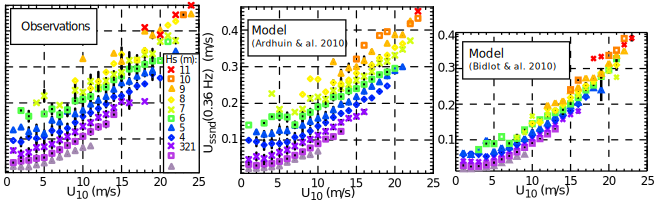
\includegraphics[width=1.0\textwidth]{FIGS_CH_MODEL/Ussnd_46005.pdf}}
  \caption{Surface Stokes drift for all wave components with a frequency below 0.36~Hz, 
  at the location of NOAA buoy 46005, off the U.S. West Coast.
  In this calculation we have assumed that all waves travel in the same direction, giving 
  a non-directional Stokes drift $U_{ssnd}$. The true directional 
  spreading typically gives a true Stokes drift that is  15\% less. 
  Observed and modeled values were binned as a function of wind speed $U_{10}$ and wave height. For each bin, the 
  mean value is plotted and the black bars represent half the standard deviation of the bin. 
  We find that over 90\% of the variance of 
  $U_{ssnd}$ is explained by $U_{10}$ and $H_s$.
  When using the parameterization by \cite{Bidlot&al.2005}, the variability is not well reproduced. }
  \label{Ussnd}
\end{figure}
%%%%%%%%%%%%% end of figure
Hence, an empirical approximation that gives $U_{ss}$ as a function of $H_s$ and wind speed can be a better 
choice than some model results \citep[see eq. (C3) in][]{Ardhuin&al.2009}.

